\section{Datenspeicherung}
Da eine grosse Datenmenge zusammenkommen kann, welche gespeichert werden muss, ist es sinnvoll eine $\mu$SD-Karte zu nehmen. Diese muss dann vom Arduino Mega aus beschrieben und gelesen werden können. Die Kosten dafür sind sehr gering gehalten, da der Storage Adapter nur wenige CHF kostet (<5CHF) und auch die $\mu$SD-Karte sehr günstig zu beziehen ist (ca. 20CHF für 64GB). Die Beschreibung der $\mu$SD-Karte würde allerdings dann ein Textfile generieren, welches mit einem Adapter für den PC selbst direkt ausgegeben werden kann. Somit sind generell jegliche Loggdaten der Wetterstation nichtflüchtig speicherbar.
\begin{figure}[hbtp]
\centering
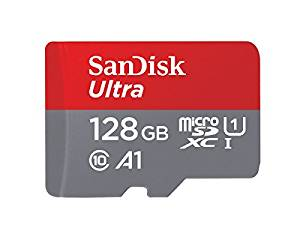
\includegraphics[width=0.7\textwidth]{graphics/msdcard.jpg}
\caption{Je nachdem abhängig, was der Storage Adapter unterstützt.}
\end{figure}
